% act_1.2
\subsection{Step reference generation}
The objective of this activity is display the UR5 robot on rviz. The simulation should start with the initial joint configuration $\begin{bmatrix} \pi & -\frac{\pi}{8} & -\frac{\pi}{6} & 0.0 & 0.0 & 0.0 \end{bmatrix}$ and then move the second and fifth joint. The joints will maintain the initial configuration during the first $2$ seconds and follow a step reference during the last $3$ seconds. The function to generate the step reference is describe in Algorithm \ref{lst:step_reference_generator} and the rosnode file to move the second and fifth joint of UR5 robot is describe in Algorithm \ref{lst:rosnode_step_reference_generator}. Finally, Figure \ref{fig:act_1.2_joint_position}-\ref{fig:act_1.2_joint_acceleration} shows the joint position, velocity and acceleration of each joint of the UR5 robot.

\begin{lstlisting}[language=Python,caption=Function to generate step reference., label={lst:step_reference_generator}]
def step_reference_generator(a):
    """
    Info: generate a constant reference.

    Inputs:
    ------
        - a: constant reference
    Outputs:
        - constant signal 
    """
    q = a       # [rad]
    dq = 0      # [rad/s]
    ddq = 0     # [rad/s^2]
    return q, dq, ddq
\end{lstlisting}



\begin{lstlisting}[language=Python, caption={Rosnode to move the second and fifth joint of UR5 robot with the requirement motion of activity 1.2.}, label={lst:rosnode_step_reference_generator}]
# =========================
#   Configuration of node
# =========================
# create a node: 
rospy.init_node("node_sinusoidal_reference_generation")

# public in topic /joint_states	to send joint data	
pub = rospy.Publisher('joint_states', JointState, queue_size=1000)

# loop rate (in Hz)
rate 	= rospy.Rate(100)		# 100 [Hz]
dt 		= 1e-2					# 10  [ms]

# joints name of UR5 robot
jnames = ['shoulder_pan_joint', 'shoulder_lift_joint', 'elbow_joint','wrist_1_joint', 'wrist_2_joint', 'wrist_3_joint']

# object(message) type JointState
jstate = JointState()

# ==========================================
#   Set initial joint configuration of UR5
# ==========================================
# initial configuration: position, velocity and acceleration 
q0 =   np.array([np.pi, -np.pi/8,  -np.pi/6, 0.0, 0.0, 0.0])
qd0 =  np.array([    0.0, 0.0, 0.0, 0.0, 0.0, 0.0])
qdd0 = np.array([    0.0, 0.0, 0.0, 0.0, 0.0, 0.0]) 

# desired trajectory: position, velocity and acceleration
q_des = np.zeros(6)
dq_des = np.zeros(6)
ddq_des = np.zeros(6)

#===============
#   Simulation
#===============
t = 0.0                     # [sec] 
simulation_duration = 5.0   # [sec]
step_start = 4.0            # [sec]

while not rospy.is_shutdown():
    # generate step reference after 2 seconds
    if t>=step_start:
        # second link
        q_des[1], dq_des[1], ddq_des[1] = step_reference_generator(-0.4)
        # fifth link
        q_des[4], dq_des[4], ddq_des[4] = step_reference_generator(-0.5)

    # publish message
    jstate.header.stamp = rospy.Time.now()
    jstate.name 		= jnames			# Joints position name
    jstate.position 	= q_des
    jstate.velocity 	= dq_des
    pub.publish(jstate)

    # update time
    t = t + dt
    
    # stop simulation
    if t>=simulation_duration:
        print("stopping rviz ...")
        break
    rate.sleep()

\end{lstlisting}


\begin{figure}
    \centering
    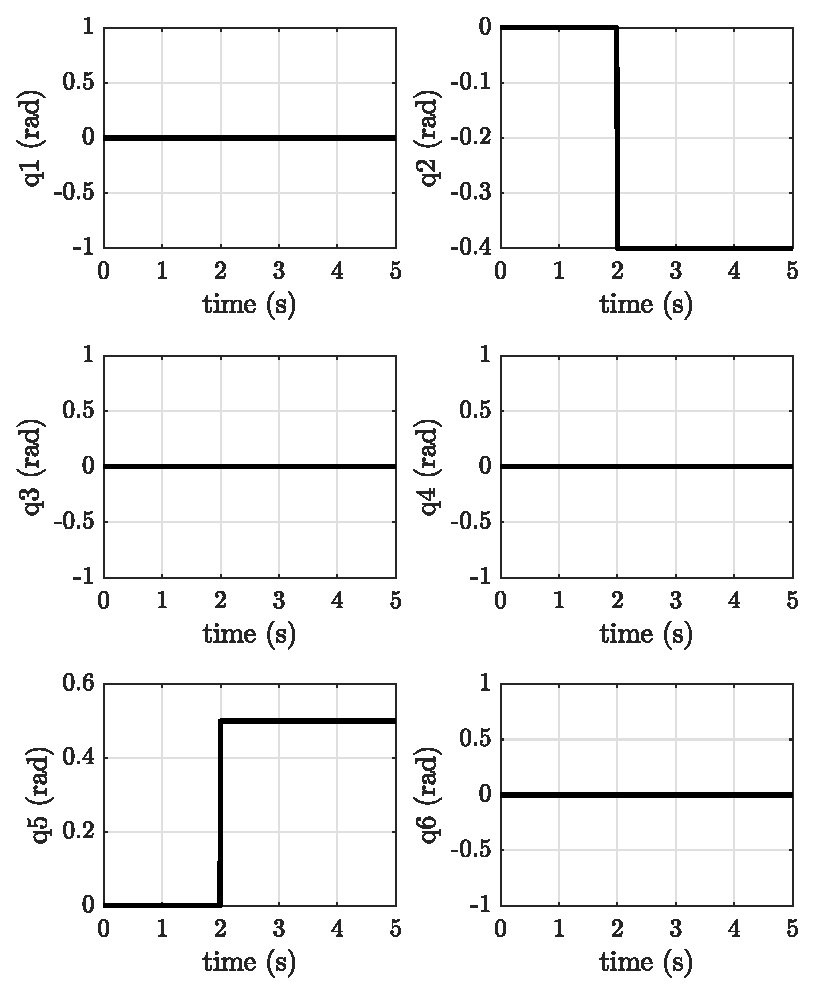
\includegraphics{images/act_1.2/joint_position.eps}
    \caption{Angular position of each joint of UR5 robot with Algorithm \ref{lst:rosnode_sine_reference_generator}.}
    \label{fig:act_1.2_joint_position}
\end{figure}

\begin{figure}
    \centering
    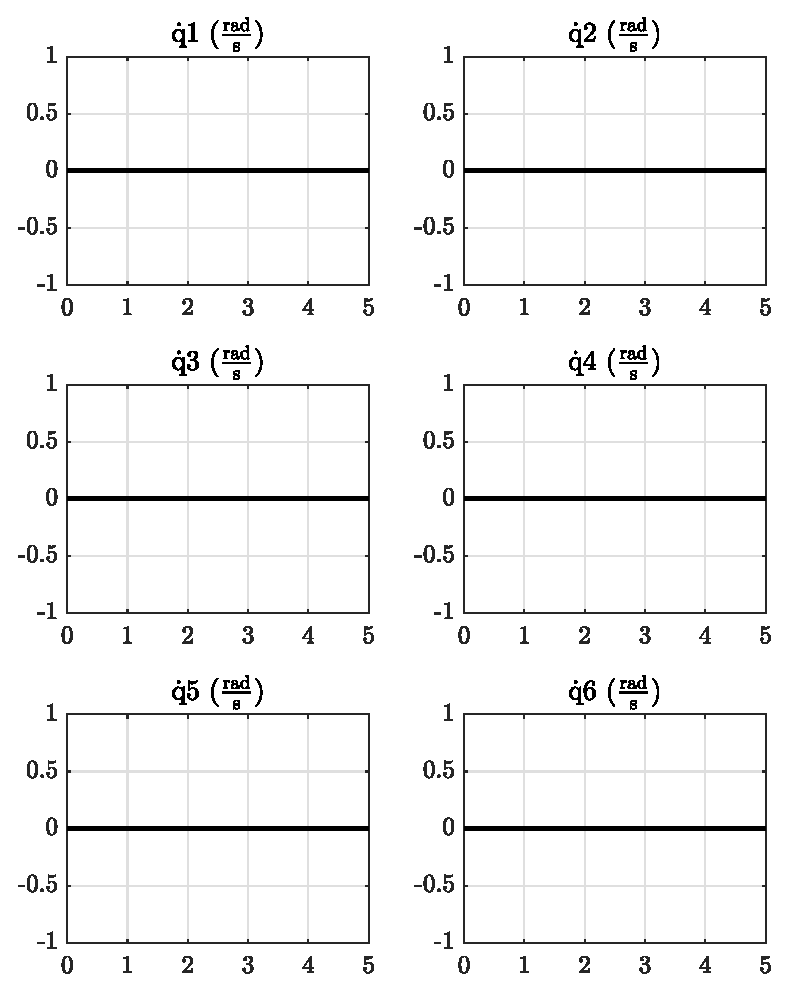
\includegraphics{images/act_1.2/joint_velocity.eps}
    \caption{Angular velocity of each joint of UR5 robot with Algorithm \ref{lst:rosnode_sine_reference_generator}.}
    \label{fig:act_1.2_joint_velocity}
\end{figure}

\begin{figure}
    \centering
    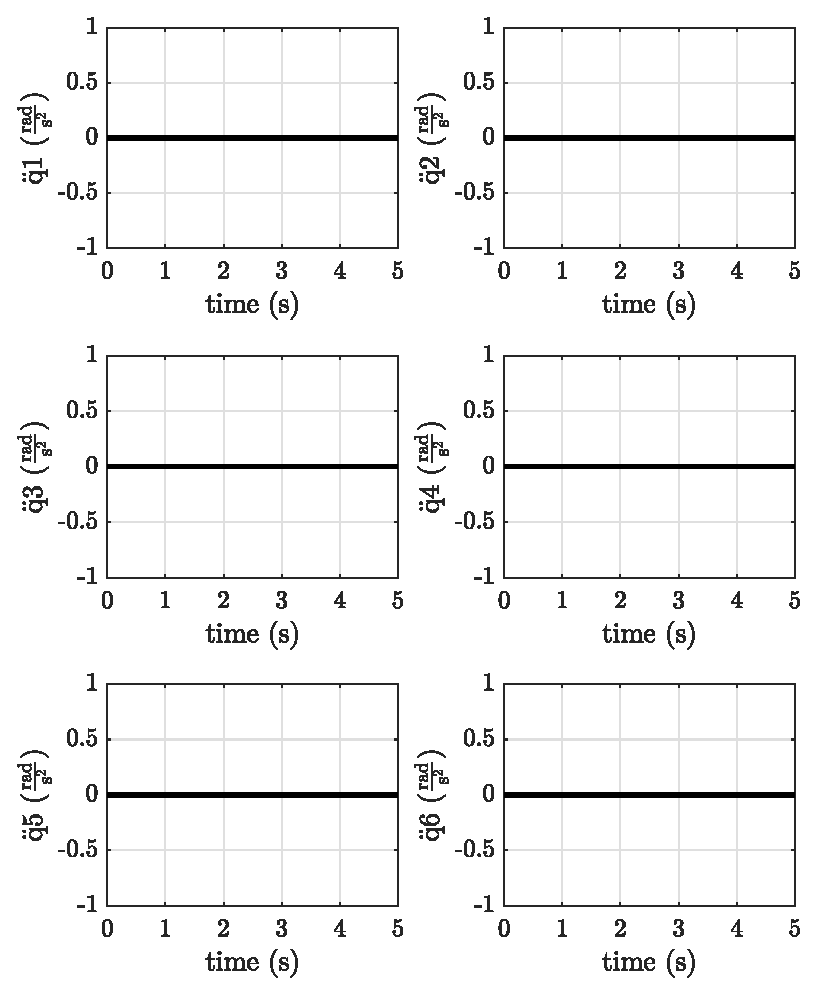
\includegraphics{images/act_1.2/joint_acceleration.eps}
    \caption{Angular acceleration of each joint of UR5 robot with Algorithm \ref{lst:rosnode_sine_reference_generator}.}
    \label{fig:act_1.2_joint_acceleration}
\end{figure}